\section*{Appendix overview}
{This appendix is organized to follow the evidence chain of the paper.}
{\textbf{\S\ref{app:benchmark}} documents benchmark construction and the per-category/domain heatmap used by the main text.}
{\textbf{\S\ref{app:failure_ext}--\S\ref{app:eval_correlation}} provide focused failure-analysis context and judge--human agreement.}
\textbf{\S\ref{app:full_component_breakdown}} gives the full nine-component score breakdown across all generators.
\textbf{\S\ref{app:prompts}--\S\ref{app:eval}} provide the end-to-end workflow, reasoner I/O examples, and evaluation protocol.
\textbf{\S\ref{app:hardware}} documents hardware and training/serving implementation details.
\textbf{\S\ref{app:limitations}--\S\ref{app:broader}} summarize limitations, release safeguards, third-party/API caveats, and broader impact.
\section{Benchmark and dataset details}
\subsection{Benchmark construction details}
\label{app:benchmark}
\textbf{Taxonomy annotation reliability.}
Two annotators independently labeled 2{,}000 sampled failure cases, iteratively
refined the schema to Cohen's $\kappa > 0.85$, then applied it to all
10{,}840 prompts in the production scrape.
The taxonomy's stability across annotators supports viewing it as capturing
structure in the failure space rather than an artifact of labeling choices.

The failure taxonomy appears in Table~\ref{tab:taxonomy} (main paper).

\begin{figure}[t]
\centering
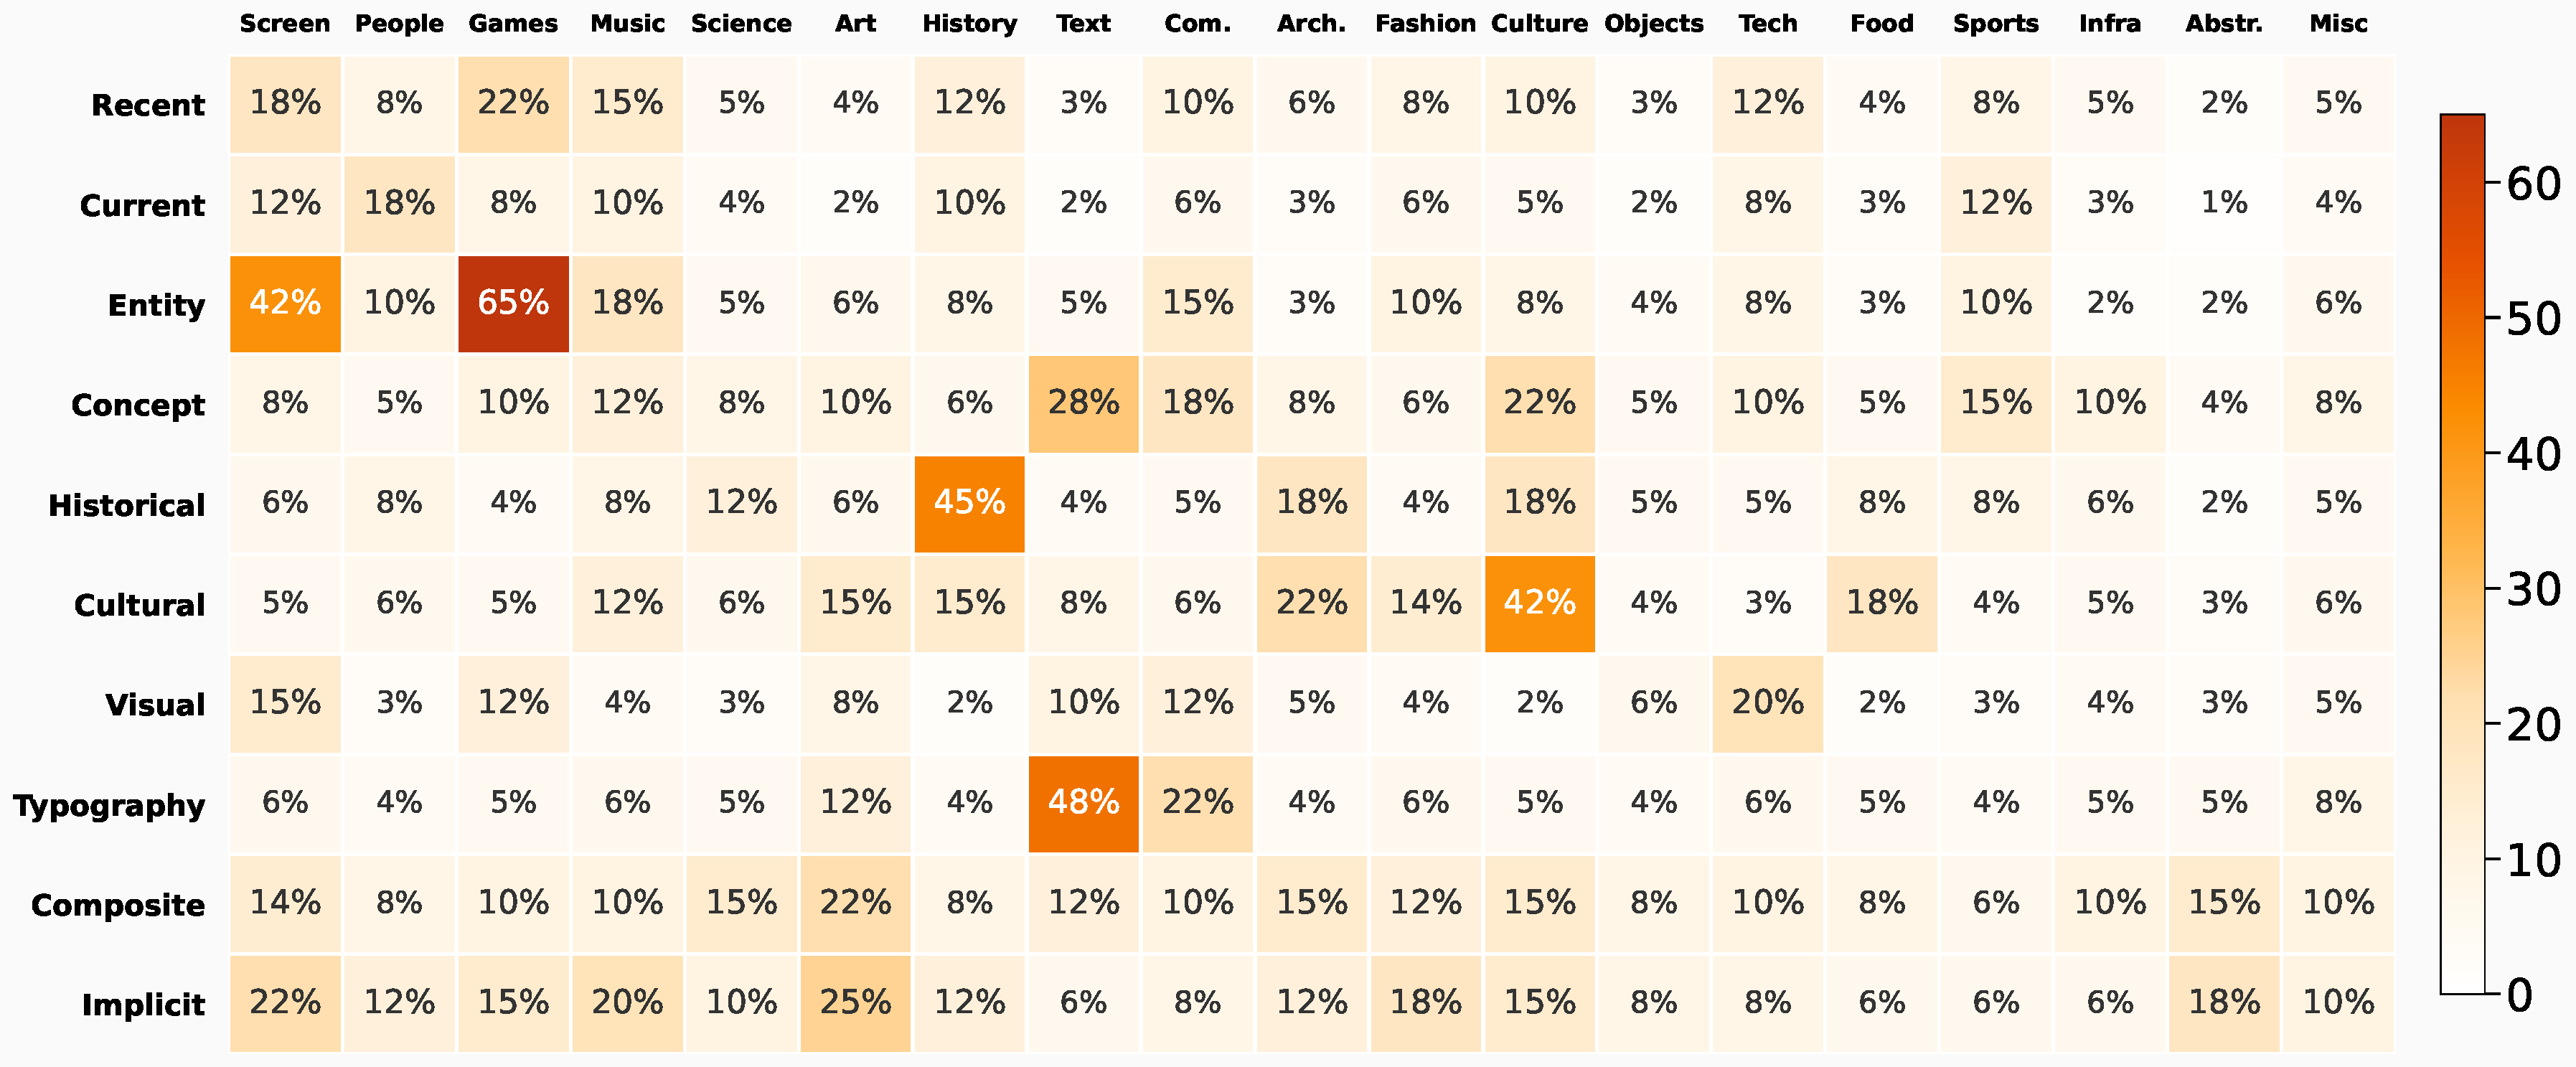
\includegraphics[width=0.85\linewidth]{figures/heatmap.pdf}
\caption{\small\textbf{The bottleneck is pervasive: every domain--category combination shows knowledge-driven degradation.}
Heatmap summarizing cross-category structure between failure modes and domain categories in \dataset{}. The uniform severity across all cells rules out the hypothesis that failures concentrate in a few niche categories.}
\label{fig:heatmap_severity}
\end{figure}

\textbf{Layer 1 (seed entities).}
From the 10{,}840 real user prompts, we extract a seed database of
31{,}537 entities spanning 22 primary domains, each annotated with canonical
name, estimated training-set frequency, ground-truth visual references, and
distinguishing attributes. The distribution is intentionally long-tailed,
mirroring real user demand.

\textbf{Layer 2 (prompt synthesis).}
From the seed database, we synthesize the \dataset{} corpus in three steps.
First, \emph{template instantiation} produces structured drafts across categories and domains by filling parameterized slots for entities, relations, and stylistic constraints distilled from the production scrape.
Second, a \emph{frontier large language model} rewrites each instantiated template into a naturalistic user-style request while preserving grounded entities, modality requirements (image versus text retrieval), and checklist-eligible facts; temperature is elevated to diversify surface form and reduce templating artifacts.
Third, \emph{quality control} removes prompts that are ambiguous under the evaluation protocol, culturally insensitive, or misaligned with the intended failure mode; annotators also verify that checklist items remain answerable from the prompt and cached search evidence alone.
Each accepted prompt includes 2--4
ground-truth search queries, a structured list of 3--8 key visual elements
with binary verification checklists, and a 1--5 evaluation rubric tailored
to the failure category. This annotation infrastructure enables fully
automated evaluation via a Gemini-3-Flash VLM judge~\cite{nanobanana2025gemini} (Spearman $\rho = 0.87$ with human
ratings; methodology in Appendix~\ref{app:eval_correlation}).

\textbf{Cultural diversity and splits.}
The benchmark spans global cultural diversity---entities from East Asia,
South Asia, the Middle East, Africa, Latin America, and beyond---because
knowledge gaps concentrate in long-tail cultural concepts and a
Western-centric benchmark would underestimate severity. For supervised
training and model selection we use train (20{,}000), validation (128), and
\textbf{test} (751) partitions, matching Section~\ref{sec:bench_construct}; remaining non-test prompts support cached
search construction, trajectory collection, and co-training rollouts.
Unlike benchmarks that test compositionality within known
concepts~\cite{genaibench,t2icompbench,dalleval}, \bench{} targets
knowledge absence.
\section{Additional empirical analysis}
\subsection{Extended failure analysis}
\label{app:failure_ext}

\textbf{Concept corruption (gating).}
The generator's conditioning architecture typically has no reliable mechanism
for gating external information based on its own confidence in its internal
representation. When a reference image (or strongly textually specified
exemplar) is provided, it is integrated with substantial weight regardless
of whether the generator's native rendering would have been more accurate
on the same entity, yielding concept corruption on prompts where internal
knowledge was already adequate.

\textbf{Reference copying (pixel-level conditioning).}
Visual conditioning operates on pixel (and low-level feature) statistics rather
than explicit semantic attributes. Without an integration layer that specifies
which attributes to transplant, the generator tends to reproduce incidental
structure from the reference---background, lighting, framing---so the output
resembles a filtered search result rather than a new composite generation.

\textbf{Why surface cues are a poor proxy for Qwen-Image-boundary strata.}
Named entities and other shallow triggers are only loosely correlated with
the knowledge boundary inferred from Qwen-Image in Table~\ref{tab:bottleneck_overall}: many
prompts contain proper nouns that already lie inside Qwen-Image's \emph{NoSearch}
stratum, while some high-gap prompts yield few detectable entities. Cheap
gates therefore trigger search on the wrong subset, repeating the same
tradeoff between \emph{VisualSearch}/\emph{TextualSearch} gains and
\emph{NoSearch} regressions that \emph{BlindSearch} exhibits outright.

\textbf{TextualSearch stratum (extended discussion).}
The main paper (\S\ref{sec:exp_strata}) compresses the TextualSearch finding: for Klein-4B-DPO, both \CondGS and \CondGAS score below the no-search baseline because internalized contextual knowledge makes search net harmful on the hardest prompts.
Those prompts disproportionately require compositional contextual reasoning---typography, cultural composition, and implicit interpretation---that resists both single-pass parameterization and single-pass search, motivating richer co-training cycles and search strategies.

\subsection{Judge--human correlation and judge--reasoner independence}
\label{app:eval_correlation}

\textbf{Human study protocol.}
Human ratings are collected on the same 500 prompt--image pairs used to report aggregate agreement in \S\ref{sec:bench_construct}.
Each pair is presented with the user prompt, the checklist, and the category rubric; raters assign checklist judgments, rubric scores, and holistic quality judgments using the same anchors as the automated judge.
Multiple raters participate with adjudication on high-disagreement items so that gold labels are stable under resampling.

\textbf{Aggregate agreement.}
The Gemini-3-Flash judge achieves Spearman $\rho = 0.87$ with the consolidated human labels on this set, which is consistent with scalable VLM-as-judge practice for text-to-image faithfulness evaluation~\cite{hu2023tifa,wiles2024gecko,lee2024heim}.

\textbf{Stratified difficulty.}
Agreement is tightest on object-centric \emph{NoSearch} prompts where errors are predominantly omissions of salient attributes.
Agreement weakens on \emph{TextualSearch}, where glyph-level correctness and fine layout dominate rubric variance; this pattern aligns with known limitations of VLMs on dense in-image text and motivates treating TextualSearch as a conservative stratum in automated evaluation.

\section{Extended quantitative results}
\label{app:extended_quant}

\subsection{Full nine-component breakdown by stratum}
\label{app:full_component_breakdown}

Table~\ref{tab:bottleneck_full} provides the complete nine-component evaluation for all generators on both the NoSearch and Search-Intensive strata.
This supplements the six-component summary in the main paper (Table~\ref{tab:bottleneck_overall}) with the full scoring breakdown.

\begin{table}[t]
\centering
\caption{\textbf{The Search Bottleneck on \bench{} -- Full Nine-Component Breakdown.}
Scores on a 0--100 scale (one decimal); higher is better.
Every generator drops sharply on the \emph{Search-Intensive} set, confirming that the bottleneck reflects missing knowledge rather than rendering ability.
Knowledge-sensitive components (Checklist, Rubric, Visual Ref.) vary per prompt and measure knowledge presence; knowledge-invariant components (Text Rend., Phys.\ Plaus., Img.\ Qual.) measure rendering competence.}
\label{tab:bottleneck_full}
\small
\setlength{\tabcolsep}{2.0pt}
\resizebox{\columnwidth}{!}{%
\begin{tabular}{@{}llcccccccccc@{}}
\toprule
\textbf{Type} & \textbf{Generator}
  & \textbf{Overall} & \textbf{Checklist} & \textbf{Rubric} & \textbf{Prompt}
  & \textbf{Img.\ Qual.} & \textbf{Text Rend.} & \textbf{AI Nat.} & \textbf{Comp.\ Aes.}
  & \textbf{Phys.\ Plaus.} & \textbf{Vis.\ Ref.} \\
\midrule
\multicolumn{12}{@{}l}{\emph{NoSearch set (parametric knowledge sufficient)}} \\
\addlinespace[2pt]
\multirow{4}{*}{Open}
& Bagel              & 49.3 & 52.3 & 49.1 & 39.2 & 58.0 & 18.4 & 48.3 & 65.3 & 60.4 & 34.8 \\
& Flux.2-Klein-4B    & 51.0 & 54.7 & 51.8 & 39.3 & 61.3 & 13.2 & 49.5 & 67.2 & 63.5 & 32.6 \\
& Flux.2-Klein-9B    & 57.8 & 63.8 & 59.8 & 51.3 & 63.8 & 31.3 & 52.5 & 72.3 & 66.7 & 43.7 \\
& Qwen-Image         & 67.4 & 74.8 & 70.8 & 62.8 & 68.3 & 63.0 & 61.0 & 76.8 & 73.8 & 56.7 \\
\midrule
\multirow{6}{*}{Commercial}
& Qwen-Image-2       & 70.7 & 78.7 & 73.8 & 68.4 & 70.2 & 71.7 & 60.8 & 80.3 & 75.6 & 60.0 \\
& SeedDream-4.0      & 67.9 & 74.9 & 70.6 & 61.7 & 69.5 & 71.1 & 59.7 & 80.3 & 73.9 & 56.7 \\
& Nano Banana        & 63.1 & 71.1 & 67.5 & 59.7 & 66.3 & 42.8 & 56.5 & 76.3 & 68.5 & 53.8 \\
& Nano Banana Pro    & 75.0 & 82.8 & 78.1 & 72.8 & 71.5 & 85.9 & 65.0 & 83.3 & 78.2 & 67.8 \\
& GPT-Image-2        & 71.1 & 78.6 & 75.6 & 70.8 & 69.0 & 67.7 & 60.8 & 77.7 & 73.9 & 64.3 \\
\midrule
\multicolumn{12}{@{}l}{\emph{Search-Intensive (external knowledge required)}} \\
\addlinespace[2pt]
\multirow{4}{*}{Open}
& Bagel              & 21.5 & 18.2 & 17.6 & 13.3 & 30.5 &  2.5 & 29.3 & 33.6 & 36.8 & 13.5 \\
& Flux.2-Klein-4B    & 24.1 & 19.8 & 18.4 & 12.4 & 37.2 &  4.2 & 33.6 & 39.3 & 46.2 & 11.9 \\
& Flux.2-Klein-9B    & 26.7 & 24.2 & 23.1 & 17.2 & 36.8 &  7.2 & 32.9 & 40.4 & 48.6 & 16.9 \\
& Qwen-Image         & 27.9 & 24.8 & 24.3 & 18.6 & 40.1 &  8.7 & 31.6 & 42.8 & 44.6 & 17.7 \\
\midrule
\multirow{6}{*}{Commercial}
& Qwen-Image-2       & 31.6 & 28.5 & 27.1 & 22.1 & 42.2 & 12.7 & 36.3 & 45.5 & 48.2 & 21.0 \\
& Imagen3-Fast       & 14.1 &  9.7 & 10.0 &  6.9 & 22.2 &  1.4 & 21.4 & 23.2 & 23.7 &  7.0 \\
& SeedDream-4.0      & 45.9 & 44.2 & 43.6 & 38.5 & 57.0 & 35.9 & 47.1 & 58.7 & 64.0 & 35.1 \\
& Nano Banana        & 44.1 & 41.0 & 40.4 & 36.0 & 57.1 & 28.0 & 47.4 & 61.5 & 65.5 & 33.2 \\
& Nano Banana Pro    & 65.3 & 64.4 & 63.1 & 60.7 & 71.4 & 65.0 & 62.0 & 75.9 & 78.5 & 58.3 \\
& GPT-Image-2        & 71.0 & 71.2 & 70.1 & 69.2 & 75.1 & 75.9 & 64.7 & 80.4 & 77.3 & 66.0 \\
\bottomrule
\end{tabular}%
}
\end{table}

\section{Protocols and supplementary artifacts}
\subsection{End-to-end workflow and reasoner I/O}
\label{app:prompts}
\label{app:reasoner_io}
% D.1 (standalone end-to-end worked example) collapsed into the reasoner I/O section:
% appendix_reasoner_io now leads with a condensed workflow overview, then the per-stage I/O.
% The full standalone worked example is retained but disabled for now:
% \input{appendix_workflow_eval025}
% Per-stage reasoner I/O (gate / filter / integrate), shown in compact structured form
% matching the main-paper evaluation-context example (examplebox), NOT verbatim JSON.
% The released co-training corpus holds the exact JSON schema; here we show the same
% fields (\texttt{...}) in a shortened, readable form.

The reasoner's three stages of \S\ref{sec:atomic}---\textbf{gate} (Stage~1),
\textbf{filter} (Stage~2), and \textbf{integrate} (Stage~3)---are stored in our SFT
corpus as trajectory types Task~A, Task~B, and Task~C, respectively.
We first trace a \emph{single} request end-to-end to show the overall inputs and outputs,
then give one representative input--output pair per stage so the input contract and output
fields (shown as \texttt{field}) are visible at a glance. We render outputs in compact
form; the released co-training corpus contains the verbatim JSON in the exact schema.
These are representative \emph{successful} cases; failure modes such as copy effects are
analyzed in \S\ref{sec:naive}.

% ============================================================
% End-to-end workflow overview (condensed; collapsed from former standalone D.1)
% ============================================================
\paragraph{End-to-end workflow (condensed).}
A user prompt enters; the reasoner runs gate\,$\to$\,filter\,$\to$\,integrate to decide
what to search, select references, and emit an enriched prompt; the generator renders the
image; and a VLM judge scores it against a checklist and rubric. The box below traces one
request through these steps, and Figure~\ref{fig:workflow_overview} shows the retrieved
references and the resulting generation.

\begin{examplebox}
\small
\textbf{End-to-end example (condensed).}\\[2pt]
\textbf{Input --- user request:} \emph{``Paint Yang Chaoyue on a 1970s Chinese rural field ridge; commune-member clothing; long-handled hoe; earth tones; 1970s film grain.''}\\[3pt]
\textbf{Stage~1 (gate) --- image search queries:} Yang Chaoyue natural photo; 1970s commune labor scene; 1970s rural film photography; long-handled hoe.\\[2pt]
\textbf{Stage~2 (filter) --- selected references:} a period rural-ridge scene; commune work clothing; Yang Chaoyue likeness.\\[2pt]
\textbf{Stage~3 (integrate) --- enriched prompt (output to generator):} \emph{``A 1970s Chinese rural labor scene on a yellow-earth field ridge: Yang Chaoyue in period commune clothing, holding a wooden long-handled hoe with a curved iron blade, natural expression, earth-tone palette, slight vintage color cast, film grain, no modern elements.''}\\[2pt]
\textbf{Output --- generation \& evaluation:} the enriched prompt and the three references condition the generator (Figure~\ref{fig:workflow_overview}); a VLM judge then scores the result on likeness, historical authenticity, and atmospheric tone (protocol in \S\ref{app:eval}).
\end{examplebox}

\begin{figure}[t]
  \centering
  \setlength{\tabcolsep}{3pt}
  \begin{tabular}{@{}ccc@{}}
    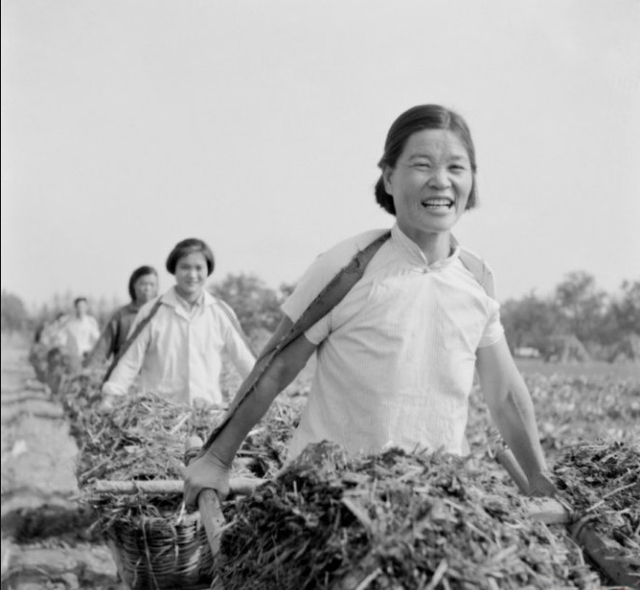
\includegraphics[width=0.30\linewidth]{figures/appendix_workflow_eval025_i2i_ref1_scene.jpg} &
    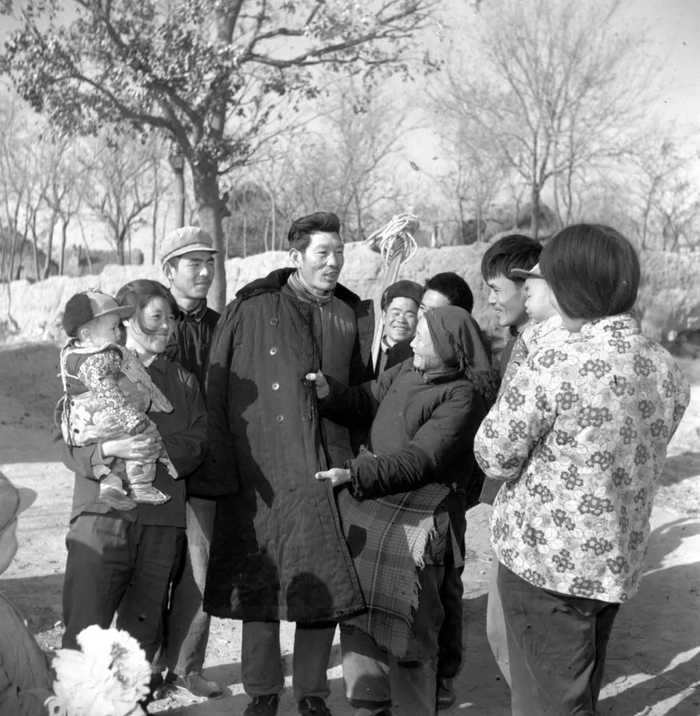
\includegraphics[width=0.30\linewidth]{figures/appendix_workflow_eval025_i2i_ref2_clothing.jpg} &
    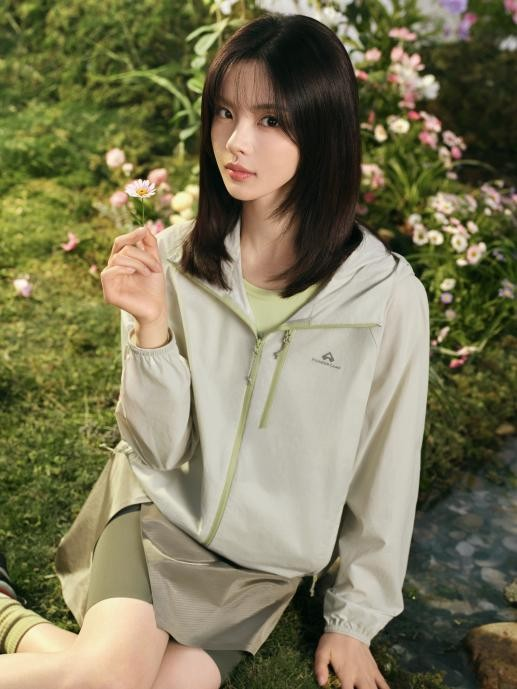
\includegraphics[width=0.30\linewidth]{figures/appendix_workflow_eval025_i2i_ref3_likeness.jpeg} \\
    \scriptsize Reference~1 (scene) & \scriptsize Reference~2 (costume) & \scriptsize Reference~3 (likeness)
  \end{tabular}\\[6pt]
  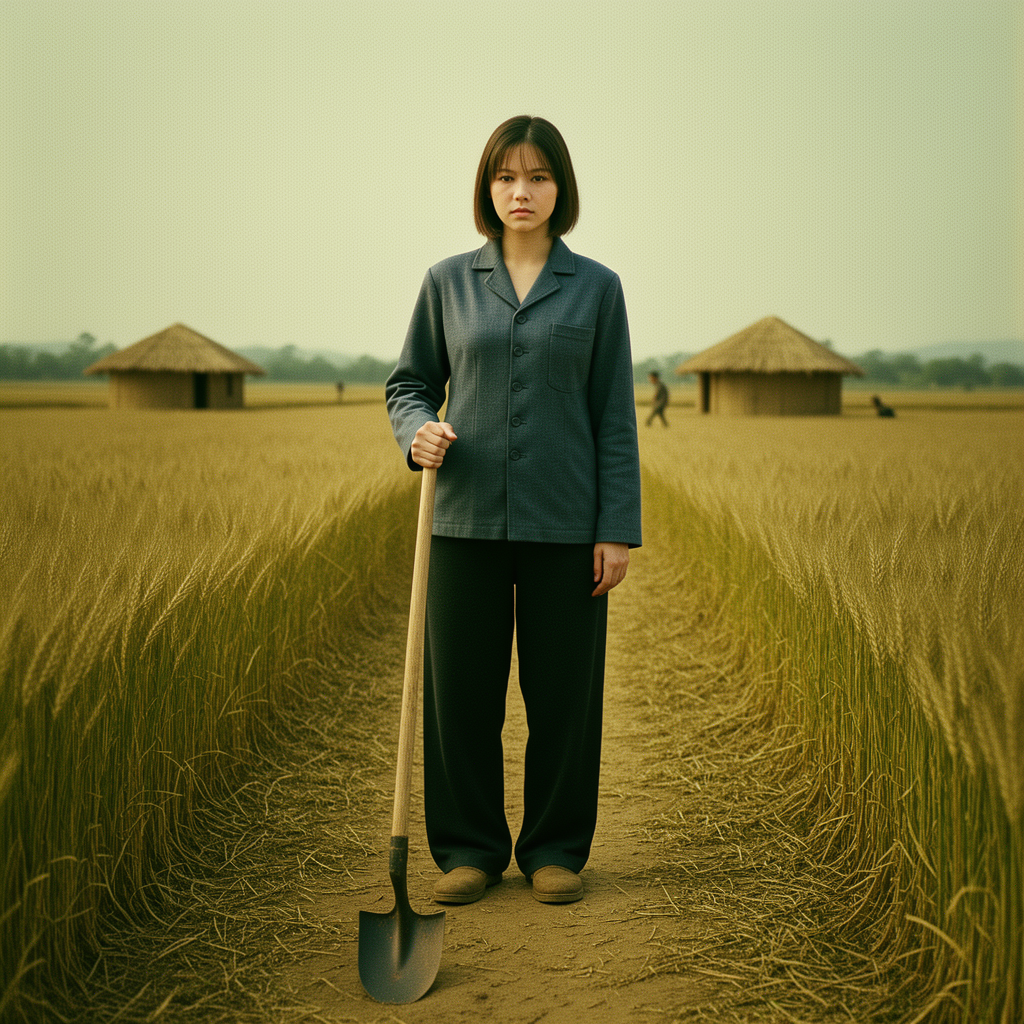
\includegraphics[width=0.55\linewidth]{figures/appendix_workflow_eval025_generated.png}\\[2pt]
  {\scriptsize Augmented output (Flux.2-Klein-4B-DPO).}
  \caption{\textbf{The end-to-end example's visual output.} The three references the reasoner
  retrieved and selected (top: scene, costume, likeness) and the image the generator produced
  from the enriched prompt (bottom), for the Yang Chaoyue request traced in the box above.
  This is the section's only image example; it grounds what ``retrieved references'' and
  ``generation'' concretely look like. The per-stage boxes that follow are text-only and use
  different prompts, each chosen to isolate one stage's behavior.}
  \label{fig:workflow_overview}
\end{figure}

% ============================================================
% Stage 1 -- Gate (Task A)
% ============================================================
\paragraph{Stage~1 --- Gate (SFT Task~A).}
The gate decides \emph{whether} external grounding is needed, classifies each surviving
gap by type and severity, and proposes modality-labeled search queries. The two cases
below show the decision it must make: it \emph{fires} on a named landmark with a critical
visual-identity gap, and it \emph{skips} a generic studio prompt the base generator
already renders reliably---the discipline that keeps the pipeline from over-retrieving.

\begin{examplebox}
\small
\textbf{Stage~1 (gate) --- search fires.}\\[2pt]
\textbf{Prompt:} \emph{``Photorealistic dusk poster of the Shanghai Tower showing its actual spiral facade and correct height proportions.''}\\[3pt]
\textbf{Knowledge gap:} Shanghai Tower --- \texttt{category}: entity identity; \texttt{severity}: \emph{critical}. The signature 120-degree spiral taper and tiered glass facade are frequently rendered incorrectly; an image reference fixes the exact geometry.\\[2pt]
\textbf{Decision} (\texttt{search\_decision}): \emph{search}. \quad \textbf{Query} (\texttt{modality}: image): ``Shanghai Tower full exterior dusk photograph''.\\[2pt]
\textbf{Justification:} a critical visual-identity gap survives analysis, so image search is warranted.
\end{examplebox}

\begin{examplebox}
\small
\textbf{Stage~1 (gate) --- search skips.}\\[2pt]
\textbf{Prompt:} \emph{``Photorealistic product shot of a blue and white porcelain teapot with bamboo motif on a marble tabletop, shallow depth of field, soft studio lighting.''}\\[3pt]
\textbf{Knowledge gaps} (\texttt{knowledge\_gaps}): none. Porcelain teapots, bamboo motifs, marble surfaces, and studio lighting all render reliably from training data; no named entities, events, or cultural specifics are present.\\[2pt]
\textbf{Decision} (\texttt{search\_decision}): \emph{skip}. No critical or important gap survives; searching would inject noise without improving accuracy.\\[2pt]
{\footnotesize\emph{Fields:} \texttt{severity}$\in$\{critical, important, moderate, minimal\}; \texttt{modality}$\in$\{image, web\}.}
\end{examplebox}

\bigskip

% ============================================================
% Stage 2 -- Filter (Task B)
% ============================================================
\paragraph{Stage~2 --- Filter (SFT Task~B).}
Once the gate fires, retrieval returns several candidate references; the filter selects
the single one that most directly fills the identified gap while minimizing extraneous
content. Below, only one of three candidates carries the required location-specific
layout, and the filter selects it by 0-based index.

\begin{examplebox}
\small
\textbf{Stage~2 (filter) --- reference selection.}\\[2pt]
\textbf{User request:} \emph{``Create a photorealistic render of the current Atlanta, GA UV index dashboard, showing both the real-time UV reading and the daily maximum forecast value.''}\\[2pt]
\textbf{Search query:} ``Official Atlanta Georgia real-time UV index dashboard example''.\\[3pt]
\textbf{Candidates} (0-based):
\begin{itemize}[leftmargin=1.2em,itemsep=1pt,topsep=1pt,parsep=0pt]
  \item[0.] generic Home Assistant UV-index card (dashboard widget)
  \item[1.] Atlanta, GA real-time UV index dashboard
  \item[2.] Buckhead dermatology clinic UV-safety page
\end{itemize}
\vspace{1pt}
\textbf{Identified gap} (\texttt{identified\_knowledge\_gaps}): the model lacks the location-specific layout, branding, and data structure of a real-time UV dashboard for Atlanta.\\[2pt]
\textbf{Selected} (\texttt{selected\_index}): \textbf{1}. Only candidate~1 shows an Atlanta-specific dashboard with the correct layout; candidates~0 and~2 are a generic widget and a clinical page and lack the required city-specific structure.
\end{examplebox}

\bigskip

% ============================================================
% Stage 3 -- Integrate (Task C)
% ============================================================
\paragraph{Stage~3 --- Integrate (SFT Task~C).}
The final stage folds the selected reference(s) into a generation-ready prompt, routing
visual grounding \emph{through language}: rather than passing raw pixels alone, the
reasoner names exactly what to borrow with a grounded citation (``following Image~1,
render~\dots'') so the generator inherits the missing knowledge without copying
unrequested style or layout.

\begin{examplebox}
\small
\textbf{Stage~3 (integrate) --- reference-grounded refinement.}\\[2pt]
\textbf{User request:} \emph{``Generate a photorealistic image of a polar bear standing in the Sahara Desert, looking confused as it searches for ice, with sand dunes and a single dead acacia tree nearby.''}\\[2pt]
\textbf{Reference~1:} a dead acacia tree under hard desert sunlight (retrieved for the tree's branching structure).\\[3pt]
\textbf{Borrow from Image~1} (\texttt{borrow\_from\_references}): the acacia tree's forked branching silhouette, dry cracked bark texture, and hard midday desert lighting.\\[2pt]
\textbf{Create new} (\texttt{create\_new}): the confused polar bear searching for ice; rolling Sahara dunes to the horizon; clear blue sky.\\[2pt]
\textbf{Refined prompt} (\texttt{refined\_prompt}): \emph{``Photorealistic 8k polar bear in the Sahara, furrowed brow as it searches for ice. \underline{Following Image~1}, render the dead acacia tree with the same forked branches, dry cracked bark, and hard midday sunlight; match that lighting on the bear so its white fur casts the same sharp shadows. Golden-orange dunes roll to the horizon under a clear blue sky.''}
\end{examplebox}




\subsection{Evaluation protocol}
\label{app:eval}
% Automated judge protocol (description precedes abbreviated figures).

\paragraph{Automated judge protocol.}
Each evaluation instance gives the judge the user prompt, the verification checklist, and the category-specific rubric, together with any reference images carrying short textual annotations (entity focus and severity).
References are used only as comparison evidence; the single ``image to assess'' is scored.
The judge follows a fixed sequence: recover task requirements; separate reference versus scored roles; extract observable evidence (subjects, attributes, scene, style, in-image text, artifacts); compare against references where checklist items depend on them; assign anchored half-point scores for checklist rows, rubric dimensions, and generic quality axes; then emit scored blocks for reference alignment, checklist, rubric, visual-reference fidelity, and text-reference fidelity, suitable for aggregation into the nine reported components (Table~\ref{tab:judge_components}).

% --- eval_protocol box commented out: orphaned (0 refs), its 8 steps duplicate the prose
%     paragraph directly above, and its C3-convertase example is off-theme vs. the rest of
%     the paper. Re-enable if a concrete judge-input box is wanted.
\iffalse
\begin{tcolorbox}[appevalbox, title={Evaluation Protocol: Judge Prompt Structure (abbreviated)}]
\textbf{Image layout:}\\
Reference image 1: \texttt{\textless image\textgreater} --- entity=\texttt{Annotated C3 convertase pathway schematic}, severity=\texttt{critical}\\
Reference image 2: \texttt{\textless image\textgreater} --- entity=Mature C3 $\alpha$/$\beta$ chains post-furin cleavage, severity=\texttt{important}\\
Image to assess: \texttt{\textless image\textgreater}\\[4pt]
\textbf{Evaluation steps} (8 steps, enforced in order):\\
1.~Task understanding: map user\_prompt, checklist, rubric, references\\
2.~Image roles: reference = comparison only; assessed = scored\\
3.~Evidence extraction: 11 observable categories\\
4.~Reference comparison\\
5.~Scoring: 0--3 in 0.5 steps with \textbf{auditable reason format}:
Anchor $\to$ Adjustments $\to$ Computed final\\
6.~Score all checklist items + task-specific rubric + 6 generic
dimensions\\
7.~Visual/text reference fidelity\\
8.~Consistency checks\\[4pt]
\textbf{Output:} scored blocks for reference alignment, checklist, rubric,
visual-reference fidelity, and text-reference fidelity.
\end{tcolorbox}
\captionof{figure}{Abbreviated evaluation protocol; full judge prompt ships with the supplementary materials.}
\label{fig:eval_protocol}
\fi

% --- "Illustrative parsed output" block commented out per request (prose + output box). ---
\iffalse
\paragraph{Illustrative parsed output.}
For every scored item---a checklist question, a rubric dimension, or a generic quality
axis---the judge emits a half-point score and a short auditable reason.
Figure~\ref{fig:eval_output} shows this output format on an example generation.

\begin{tcolorbox}[appscorebox, title={Evaluation Output Example (Parsed, abbreviated)}]
{\footnotesize
\setlength{\tabcolsep}{4pt}
\renewcommand{\arraystretch}{1.15}
\begin{tabularx}{\linewidth}{@{}p{2.4cm}cX@{}}
\toprule
\textbf{Item} & \textbf{Score} & \textbf{Reason} \\
\midrule
Pyramid silhouette & 1 / 3 & Slope angle is plausible, but limestone-casing detail is missing. \\
Camel anatomy & 2 / 3 & Limbs are coherent with minor hump-proportion drift. \\
Poster style & 2 / 3 & Palette evokes mid-century travel art, but composition is only partly period-authentic. \\
Lighting coherence & 3 / 3 & Golden-hour direction and shadows are consistent. \\
\bottomrule
\end{tabularx}
\par}
\end{tcolorbox}
\captionof{figure}{\textbf{Judge output format.} Each scored item carries a $0$--$3$ score
and a one-line reason; the overall score aggregates these rows into the nine reported
components (Table~\ref{tab:judge_components}).}
\label{fig:eval_output}
\fi

\bigskip

\paragraph{Score components and aggregation.}
All scores use a $[0,3]$ scale in $0.5$ steps ($0$~=~not met/contradicted, $1$~=~weak with major issues, $2$~=~mostly met with minor issues, $3$~=~fully met).
Each score is accompanied by an auditable reason in three parts: \emph{Anchor} (initial score with evidence), \emph{Adjustments} (signed deltas with justification), and \emph{Computed final} (clamped sum matching the emitted score).
Table~\ref{tab:judge_components} lists the nine reported components and their judge instructions.
The overall score is the mean of present components, rescaled to $0$--$100$.

\begin{table}[h]
\centering
\caption{\textbf{Judge scoring components.} Each component is scored on $[0,3]$. Components 1--2 are prompt-specific; components 3--8 are fixed generic dimensions scored for every image; component 9 is conditional on whether reference images are provided.}
\label{tab:judge_components}
\small
\renewcommand{\arraystretch}{1.25}
\begin{tabularx}{\linewidth}{@{}clX@{}}
\toprule
\textbf{\#} & \textbf{Component} & \textbf{Judge instruction (abbreviated)} \\
\midrule
1 & Checklist & Mean of per-item verification scores. Each prompt carries 3--10 binary-verifiable items (e.g., ``Is the Om symbol correctly formed?''); the judge scores each against observable evidence. \\
2 & Rubric adaptive & Weighted mean of prompt-specific rubric dimensions (e.g., \emph{symbol\_accuracy}, \emph{historical\_fidelity}) excluding the six fixed generic dimensions below. \\
\midrule
3 & Prompt faithfulness & Are all requested subjects, attributes, actions, scene, and style present and accurate? \\
4 & Image quality & Visual clarity and sharpness; absence of artifacts or defects; style, lighting, and perspective coherence. \\
5 & Text rendering & Does rendered in-image text match required content? Readable, correctly spelled, well-placed? Score left empty if no text is required and none is present. \\
6 & AI naturalness & Organic texture realism vs.\ AI smoothness; fine-detail plausibility vs.\ uncanny uniformity; environment grounded vs.\ dreamlike or generic. \\
7 & Composition \& aesthetics & Framing and balance; depth and spatial arrangement; color harmony and consistent lighting; overall visual appeal. \\
8 & Physical plausibility & Anatomy (fingers, limbs, proportions, pose); object physics (gravity, support, balance); spatial consistency (perspective, scale, occlusion); material properties; lighting and shadow consistency. Score left empty for abstract or stylized content. \\
\midrule
9 & Visual reference fidelity & Scored only when reference images are attached. Identity preservation (facial features, distinguishing traits); attribute consistency (colors, textures, proportions); style fidelity. Skipped (not zero) when no references are provided. \\
\bottomrule
\end{tabularx}
\end{table}

\paragraph{Difficulty partition (Set~I--III).}
The 651 search-intensive prompts are partitioned into three difficulty sets using Nano Banana Pro no-search quality as the sorting variable: each prompt receives an overall score from Nano Banana Pro \emph{without any retrieval augmentation}, and tercile boundaries on this score distribution define Set~I (easiest third), Set~II, and Set~III (hardest third).
The partition is fixed across all experiments; the 100-prompt NoSearch subset is reported as a separate column.

\paragraph{Judge fidelity.}
The judge achieves Spearman $\rho = 0.87$ with human ratings on a
held-out set of 500 prompt--image pairs
(Appendix~\ref{app:eval_correlation}). The Anchor/Adjustment/Computed
diagnostic encourages falsifiable critiques of individual scores.


\section{Hardware and implementation details}
\label{app:hardware}
All experiments were conducted on NVIDIA H20 (80~GB HBM3) GPUs.
Below we detail the compute configuration for each training phase.

\subsection{VLM reasoner training (Phase~0 and Phase~2)}
The VLM reasoner (Qwen3-VL-8B) is trained using the ModelScope-Swift framework (\texttt{ms-swift}).
We perform full-parameter supervised finetuning with the configuration in Table~\ref{tab:app_reasoner_sft}.

\begin{table}[t]
  \centering
  \caption{\textbf{VLM reasoner SFT hyperparameters} (Phase~0 and Phase~2).}
  \label{tab:app_reasoner_sft}
  \small
  \begin{tabularx}{\linewidth}{lX}
    \toprule
    \textbf{Hyperparameter} & \textbf{Value} \\
    \midrule
    Base model & Qwen3-VL-8B-Instruct \\
    Training type & Full-parameter SFT \\
    Precision & bfloat16 \\
    Epochs & 5--6 \\
    Learning rate & $1\times 10^{-5}$ \\
    Warmup ratio & 0.05 \\
    Per-device batch size & 1 \\
    Gradient accumulation steps & 8 \\
    Effective batch size & 64 ($8$ GPUs $\times 1 \times 8$ accum.) \\
    Max sequence length & 12{,}288 tokens \\
    Max image pixels & 262{,}144 ($512^2$) \\
    Image max token number & 512 \\
    Attention implementation & FlashAttention-2 \\
    Sequence packing & Enabled (padding-free) \\
    Gradient checkpointing & Enabled \\
    ViT parameters & Frozen \\
    DeepSpeed stage & ZeRO-2 \\
    Hardware & $8 \times$ NVIDIA H20 (80~GB) \\
    Training data & ${\sim}20$K SFT trajectories \\
    Wall-clock time & ${<}4$~hours \\
    \bottomrule
  \end{tabularx}
\end{table}

The SFT dataset consists of approximately 20{,}000 expert-annotated reasoning trajectories for the gate--filter--compress pipeline (Tasks A/B/C), stored in the training-row format consumed by ModelScope-Swift.
A 1\% held-out split is used for validation.
We use dataset preprocessing with 200 workers and 4 dataloader workers for efficient data loading.

\subsection{Generator DPO training (Phase~1)}
Online iterative DPO for the visual generator (Flux.2-Klein-4B) is conducted using the Flow-Factory framework with the configuration in Table~\ref{tab:app_dpo}.

\begin{table}[t]
  \centering
  \caption{\textbf{Generator DPO hyperparameters} (Phase~1).}
  \label{tab:app_dpo}
  \small
  \begin{tabularx}{\linewidth}{lX}
    \toprule
    \textbf{Hyperparameter} & \textbf{Value} \\
    \midrule
    Base model & Flux.2-Klein-4B \\
    Finetuning type & LoRA \\
    LoRA rank / alpha & 64 / 128 \\
    Target modules & Default (attention layers) \\
    Precision & bfloat16 \\
    Learning rate & $1\times 10^{-4}$ \\
    Optimizer & AdamW ($\beta_1{=}0.9$, $\beta_2{=}0.999$, $\varepsilon{=}10^{-8}$) \\
    Weight decay & $1\times 10^{-4}$ \\
    Max gradient norm & 1.0 \\
    Resolution & $512 \times 512$ \\
    Condition image size & $512 \times 512$ \\
    Per-device batch size & 1 \\
    Group size (candidates per prompt) & 5 \\
    Unique samples per epoch & 64 \\
    Gradient steps per epoch & 2 \\
    Gradient accumulation & Auto (computed from group size) \\
    DPO $\beta$ & 100.0 \\
    Reference model device & CPU (offloaded) \\
    Advantage aggregation & Group-relative DPO \\
    EMA decay / update interval & 0.99 / 4 steps \\
    Guidance scale & 4.0 \\
    Inference steps (sampling) & 50 \\
    Timestep sampling & Logit-normal ($\mu{=}0.0$, $\sigma{=}1.0$) \\
    Gradient checkpointing & Enabled \\
    Hardware & $8 \times$ NVIDIA H20 (80~GB) \\
    Training data & ${\sim}7$K prompt--image preference pairs \\
    Save frequency & Every 10 gradient steps \\
    \bottomrule
  \end{tabularx}
\end{table}

The DPO reward signal is provided by the Qwen3-VL-8B VLM judge, served via vLLM on a separate node (accessed at inference time over HTTP).
The judge evaluates generated candidates using the \dataset{} evaluation protocol with nine scoring dimensions.
Judge inference uses a maximum of 4{,}096 output tokens, temperature 0.2, and a maximum pixel budget of 262{,}144 per image, with up to 24 concurrent requests.

\paragraph{Preference construction.}
For each prompt, the generator produces 5 candidate images (one additional candidate beyond the group for preference diversity via \texttt{preference\_extra\_candidates: 1}).
Candidates are scored by the VLM judge, and preference pairs are constructed from the highest- and lowest-scored generations within each group.
A structural similarity (SSIM) penalty (\texttt{dpo\_penalize\_condition\_ssim: 0.95}) discourages degenerate pairs where chosen and rejected images are near-identical.

\paragraph{Flow-matching dynamics.}
We use a Flow-SDE scheduler with noise level 1.0, time shift 1.0, and timestep range truncated at 0.1 for stable training.

\subsection{Reasoner rejection finetuning (Phase~2)}
Phase~2 recalibrates the reasoner to the DPO-strengthened generator using rejection-sampling finetuning.
The training infrastructure is identical to Phase~0 (ModelScope-Swift, $8 \times$ H20, same hyperparameters), with the key difference that the training data consists of filtered trajectories: only reasoner rollouts that produce positive group-relative advantage (i.e., search improved the strengthened generator's output quality) are retained for training.
The full RFT cycle completes in approximately $4 \times 8 = 32$ GPU-hours.

\subsection{Total compute budget}
Table~\ref{tab:app_compute_budget} summarizes end-to-end training compute (Phase~1 GPU-hours are $8$ GPUs $\times 24$~h wall-clock).
The VLM judge service runs concurrently on a separate GPU and is not folded into the training GPU-hour totals.

\begin{table}[t]
  \centering
  \caption{\textbf{Compute budget overview.} Training GPU-hours are approximate.}
  \label{tab:app_compute_budget}
  \small
  \begin{tabular}{@{}lccc@{}}
    \toprule
    \textbf{Phase} & \textbf{GPUs} & \textbf{Wall-clock} & \textbf{GPU-hours} \\
    \midrule
    Phase~0: Reasoner SFT & $8 \times$ H20 & ${<}4$~h & ${\sim}32$ \\
    Phase~1: Generator DPO & $8 \times$ H20 & 24~h & ${\sim}192$ \\
    Phase~2: Reasoner RFT & $8 \times$ H20 & ${\sim}4$~h & ${\sim}32$ \\
    VLM Judge serving (vLLM) & $1 \times$ H20 & concurrent & --- \\
    \midrule
    \textbf{Total (training)} & --- & --- & \textbf{${\sim}256$} \\
    \bottomrule
  \end{tabular}
\end{table}

All training runs use CUDA memory optimization via \\
\texttt{PYTORCH\_CUDA\_ALLOC\_CONF=expandable\_segments:True}.
Distributed training communication uses NCCL over NVLink interconnects within each 8-GPU node.

\section{Limitations and future directions}
\label{app:limitations}
Our work deliberately prioritizes depth of insight over exhaustive optimization, and this choice opens several promising avenues for future research.

\paragraph{Iterative co-training.}
Our recipe consists of a single DPO pass followed by a single RFT pass.
While this minimal protocol already produces monotonic improvement and validates the core principle, the knowledge boundary between internalizable and contextual knowledge is unlikely to be fully resolved in one iteration.
Multi-round co-training---where the generator and reasoner alternate improvement over several cycles---could progressively sharpen this boundary and unlock additional gains.
Investigating convergence behavior, diminishing returns, and potential instability in such iterative loops is an exciting direction.

\paragraph{Generator scale and architecture.}
Our co-training experiments use a 4B-parameter generator (Flux.2-Klein-4B) and 7B-parameter generator (Bagel).
The substantial gap between our best result and frontier commercial systems suggests that larger or architecturally different generators may internalize a broader swath of knowledge, shifting the knowledge boundary and potentially changing the distribution of prompts that require search.
Studying how the internalizable/contextual split evolves across generator scales---and whether certain failure categories (e.g., temporal-recent vs.\ cultural-specificity) exhibit qualitatively different scaling behavior---would deepen understanding of the knowledge boundary as a function of model capacity.

\paragraph{Reward signals.}
Our current evaluation relies on an automated VLM judge (Gemini-3-Flash).
While it achieves strong correlation with human ratings (Spearman $\rho = 0.87$), such judges can introduce noisy rewards---a widely acknowledged issue when automated scoring substitutes for human judgment~\cite{wiles2024gecko,lee2024heim}.
The choice of DPO is intentional: it resists reward noise by selecting the best- and worst-ranked generations to construct preference pairs~\cite{rafailov2023dpo}.

\section{Broader impact}
\label{app:broader}
This work contributes positively to the research community and society in several important ways, while also carrying risks that warrant consideration.

\paragraph{Positive impacts.}
\begin{itemize}
  \item \textbf{New evaluation resources for an underserved problem.}
  \dataset{} and \bench{} fill a significant evaluation gap.
  Existing text-to-image benchmarks predominantly test prompts that fall within generators' parametric knowledge, creating an illusion of near-solved performance.
  By systematically cataloging twelve failure categories grounded in over 10{,}000 real user prompts, our benchmark surfaces a class of failures that affects daily production use but has been largely invisible to the research community.
  Making this gap measurable is a prerequisite for closing it.

  \item \textbf{A long-tailed, culturally diverse, and challenging reference-to-image dataset.}
  The released corpus of 20{,}000 prompts, spanning twenty-two domains and intentionally representing global cultural diversity---including underrepresented cultural symbols, regional artifacts, non-Latin typography, and entities from the Global South---provides a uniquely challenging testbed.
  The long-tailed entity distribution mirrors real user demand and offers the community a resource for studying knowledge-intensive generation at a scale and diversity not previously available.
  The accompanying pre-executed search results (both image and web returns) form a fully offline search environment, lowering the barrier for reproducible research on search-augmented visual generation without requiring live API access or incurring search costs.

  \item \textbf{Advancing equitable visual generation.}
  A disproportionate share of search-intensive failures affects culturally specific content: regional festivals, indigenous art forms, historical figures outside Western canons, and scripts beyond Latin.
  By explicitly benchmarking these categories and demonstrating that search-augmented generation can improve fidelity for such content, this work contributes toward more equitable visual AI that can serve diverse global users rather than only those whose cultural knowledge is well-represented in training data.

  \item \textbf{Computational accessibility.}
  The deliberately minimal co-training recipe (one DPO pass, one RFT pass, a 4B generator, an 8B reasoner, fitting in $4\times 8$ GPU hours for the RFT phase) demonstrates that meaningful progress on knowledge-intensive generation does not require frontier-scale compute, broadening access to researchers with limited resources.
\end{itemize}

\paragraph{Potential negative impacts and mitigations.}
\begin{itemize}
  \item \textbf{Misinformation risk.}
  Improving generators' ability to render specific real-world entities---public figures, cultural symbols, historical events---could lower the barrier for producing convincing visual misinformation.
  We note, however, that our benchmark explicitly includes an ``AIGC fakeness'' evaluation dimension that measures detectable artifacts, and our released assets are evaluation prompts and search results rather than trained generator checkpoints.
  We encourage downstream users to pair improved generation with provenance tracking and watermarking.

  \item \textbf{Privacy concerns.}
  Some search-intensive prompts involve public figures.
  Our dataset construction follows standard practices: all seed entities are drawn from publicly available information, and the benchmark is designed for research evaluation rather than generating deceptive impersonations.
  We will include usage guidelines with the released dataset that prohibit malicious identity synthesis.

  \item \textbf{Bias amplification.}
  While we intentionally design for cultural diversity, the search results that form part of our released offline environment inherit biases from web search engines.
  Researchers using these results should be aware that search-returned references may reflect stereotypical or incomplete representations of certain cultures, and should evaluate whether such biases propagate into generated outputs.
  {\color{white}\nocite{wang2025code,wang2025emergent,wang2025pixelreasoner,wang2025vl,wang2025reverse,wang2026badseeingbadthinking}}
\end{itemize}


\subsection{Third-party models, data access, and terms of use}
\label{app:third_party}
\textbf{Open-weight generators.}
Bagel~\cite{deng2025bagel}; FLUX.2 Klein checkpoints~\cite{blackforest2026flux2}; Qwen-Image~\cite{qwenimage}.
\textbf{Commercial APIs.}
Qwen-Image-2~\cite{qwenimage}; Gemini developer endpoints (Gemini~2.5~Flash Image, Gemini~3~Pro Image; consumer names Nano Banana / Nano Banana Pro in some regions)~\cite{nanobanana2025gemini}; ByteDance Jimeng~\cite{jimeng2025bytedance}; SeedDream 4.0~\cite{seedream2025arxiv}; Imagen 3 Fast~\cite{baldridge2024imagen3}.
Public documentation does not specify whether these endpoints internally invoke retrieval, tool use, or proprietary knowledge bases at inference time.
Consequently, high \bench{} scores for commercial systems should be interpreted as end-to-end product behavior rather than as pure comparisons to open-weight generators under identical conditioning assumptions.

\textbf{Use.}
Experiments respect each provider's publicly posted terms and documentation; releases from this work consist of prompts and cached search artifacts, not redistributed model weights or proprietary API payloads.

\subsection{Responsible release and safeguards}
\label{app:responsible_release}

\textbf{Release scope.}
\dataset{} and \bench{} are intended for research evaluation of knowledge-intensive visual generation.
The public release will include prompts, annotations, evaluation checklists, rubrics, search queries, and permissible search metadata or derived attributes, rather than raw scraped images or proprietary web content.
We do not redistribute copyrighted source images, proprietary web content, or proprietary API payloads without permission.

\textbf{Safeguards and intended use.}
To reduce copyright and safety risks, we filter or exclude unsafe search artifacts, including explicit sexual content, graphic violence, hateful or extremist material, and personally sensitive content.
The benchmark is intended for evaluating search-intensive visual generation, not for producing deceptive, infringing, or harmful content.
Users of the released assets should respect the licenses and terms of the original sources and should not use the benchmark to generate unauthorized reproductions of protected characters, brands, or individuals.
